\documentclass[aspectratio=169,11pt]{beamer}

% ============================================================
% Theme and typography
% ============================================================

\usetheme{Madrid}
\usecolortheme{default}
\usefonttheme{professionalfonts}

\setbeamertemplate{navigation symbols}{}
\setbeamertemplate{headline}{}

\setbeamertemplate{footline}{%
  \leavevmode\hbox{%
  \begin{beamercolorbox}[wd=.82\paperwidth,ht=2.7ex,dp=1.1ex,leftskip=.8em]{author in head/foot}
    CSCI 6461 --- Computer Systems Architecture (AArch64 Reference / RISC Philosophy)
  \end{beamercolorbox}%
  \begin{beamercolorbox}[wd=.18\paperwidth,ht=2.7ex,dp=1.1ex,rightskip=.8em]{date in head/foot}
    \hfill\insertframenumber/\inserttotalframenumber
  \end{beamercolorbox}}
}

\setbeamersize{
  text margin left=0.65cm,
  text margin right=0.65cm
}

\setbeamerfont{frametitle}{size=\Large, series=\bfseries}
\setbeamerfont{block title}{series=\bfseries}
\setbeamertemplate{blocks}[rounded][shadow=false]

% ============================================================
% Packages
% ============================================================

\usepackage[T1]{fontenc}
\usepackage{lmodern}
\usepackage{amsmath}
\usepackage{booktabs}
\usepackage{array}
\usepackage{tikz}

\usetikzlibrary{
  arrows.meta,
  positioning,
  shapes.geometric
}

% ============================================================
% Colors
% ============================================================

\definecolor{navy}{RGB}{24,43,68}
\definecolor{deepblue}{RGB}{45,88,130}
\definecolor{lightblue}{RGB}{235,242,250}
\definecolor{softgray}{RGB}{245,247,250}
\definecolor{darkgray}{RGB}{25,28,32}
\definecolor{gold}{RGB}{200,145,35}

\setbeamercolor{palette primary}{bg=navy, fg=white}
\setbeamercolor{palette secondary}{bg=deepblue, fg=white}
\setbeamercolor{frametitle}{bg=navy, fg=white}
\setbeamercolor{title}{fg=white}
\setbeamercolor{subtitle}{fg=white}
\setbeamercolor{author}{fg=white}
\setbeamercolor{date}{fg=white}
\setbeamercolor{titlelike}{fg=white}
\setbeamercolor{block title}{bg=deepblue, fg=white}
\setbeamercolor{block body}{bg=lightblue, fg=darkgray}
\setbeamercolor{normal text}{fg=darkgray, bg=white}

% ============================================================
% General formatting
% ============================================================

\setlength{\parskip}{0.35em}

\newcommand{\key}[1]{\textbf{#1}}
\newcommand{\bits}[1]{\texttt{#1}}
\newcommand{\hex}[1]{\texttt{0x#1}}

% ============================================================
% Metadata
% ============================================================

\title[Week 1]{
  Introduction to Computing Systems \\
  \& Binary Foundations
}

\subtitle{
  Abstraction layers, binary representation,
  and the RISC design philosophy
}

\author{
  Computer Systems Architecture
}

\date{}

% ============================================================
% Document
% ============================================================

\begin{document}

% ============================================================
% Slide 1
% ============================================================

\begin{frame}[plain]

\begin{tikzpicture}[remember picture,overlay]
\fill[navy] (current page.south west) rectangle (current page.north east);
\fill[gold] (current page.south west) rectangle ([yshift=.15cm]current page.south east);
\end{tikzpicture}

\vspace{1.0cm}

\begin{minipage}{0.82\textwidth}

{\color{gold}\large CSCI 6461 \;|\; WEEK 1\par}

\vspace{0.28cm}

{\color{white}\fontsize{24}{28}\selectfont\bfseries
 Introduction to Computing Systems \\
 \& Binary Foundations
\par}

\vspace{0.35cm}

{\color{white!80}\large
 Abstraction, representation,
 and quantitative performance
\par}

\end{minipage}

\vfill

{\color{white}\normalsize Dr. J. Burns\par}
{\color{white!70}\small Computer Systems Architecture --- AArch64 Reference Platform\par}

\vspace{0.45cm}

\end{frame}

% ============================================================
% Slide 2
% ============================================================

\begin{frame}{What Computer Architecture Studies}

\begin{itemize}
  \item Architecture is not just ``parts of a computer.'' It is the study of the \key{interface contract between software behavior and hardware implementation}.
  \item The central question: \key{What must hardware guarantee to software, and how can hardware deliver that guarantee with maximum efficiency?}
  \item Covers instruction set design, execution pipelines, memory hierarchies, and quantitative trade-offs.
  \item A functional machine is not necessarily a good machine; architecture evaluates performance, energy, silicon area, and scalability.
\end{itemize}

\begin{block}{Philosophy vs. Reference Platform}
\begin{itemize}
  \item \key{Philosophy:} \textbf{RISC} (Reduced Instruction Set Computer) principles guide our design analysis.
  \item \key{Reference Platform:} \textbf{ARM AArch64} serves as our concrete, production 64-bit architecture throughout the semester.
\end{itemize}
\end{block}

\end{frame}

% ============================================================
% Slide 3
% ============================================================

\begin{frame}{The Core Abstraction Problem}

\begin{columns}[T,onlytextwidth]

\column{0.52\textwidth}
\begin{itemize}
  \item Programmers write high-level algorithms; hardware manipulates physical voltages and currents.
  \item Abstraction layers make complex systems manageable.
  \item Each layer hides implementation details, but hidden details directly determine execution speed and efficiency.
\end{itemize}

\column{0.44\textwidth}
\begin{block}{When Abstractions Leak}
Abstractions simplify software development, but architecture explains why they leak:
\begin{itemize}
  \item Memory hierarchy latency
  \item Integer overflow \& width limits
  \item Cache line collisions
  \item Pipeline hazards \& stalls
\end{itemize}
\end{block}

\end{columns}

\end{frame}

% ============================================================
% Slide 4
% ============================================================

\begin{frame}{System Layers: From Program to Gates}

\centering

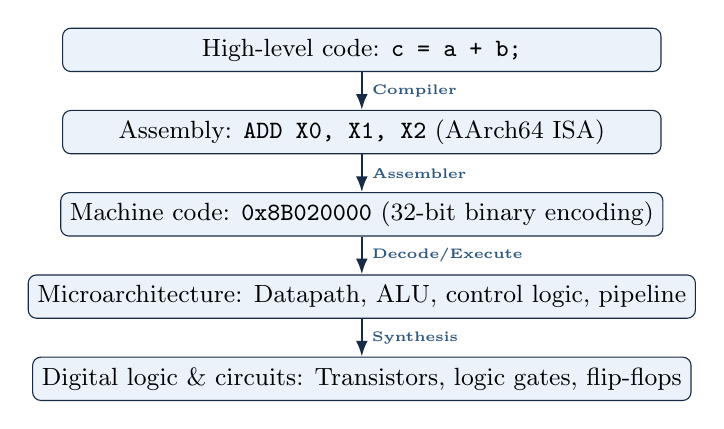
\begin{tikzpicture}[
  node distance=0.48cm,
  box/.style={
    rounded corners=3pt,
    draw=navy,
    fill=lightblue,
    align=center,
    font=\small,
    minimum width=7.6cm,
    minimum height=0.55cm
  }
]

\node[box] (c) {High-level code: \texttt{c = a + b;}};
\node[box, below=of c] (asm) {Assembly: \texttt{ADD X0, X1, X2} (AArch64 ISA)};
\node[box, below=of asm] (mc) {Machine code: \hex{8B020000} (32-bit binary encoding)};
\node[box, below=of mc] (uarch) {Microarchitecture: Datapath, ALU, control logic, pipeline};
\node[box, below=of uarch] (logic) {Digital logic \& circuits: Transistors, logic gates, flip-flops};

\draw[-{Latex[length=2mm]}, thick, navy] (c) -- (asm) node[midway, right, font=\tiny\bfseries, text=deepblue] {Compiler};
\draw[-{Latex[length=2mm]}, thick, navy] (asm) -- (mc) node[midway, right, font=\tiny\bfseries, text=deepblue] {Assembler};
\draw[-{Latex[length=2mm]}, thick, navy] (mc) -- (uarch) node[midway, right, font=\tiny\bfseries, text=deepblue] {Decode/Execute};
\draw[-{Latex[length=2mm]}, thick, navy] (uarch) -- (logic) node[midway, right, font=\tiny\bfseries, text=deepblue] {Synthesis};

\end{tikzpicture}

\end{frame}

% ============================================================
% Slide 5
% ============================================================

\begin{frame}{A Concrete Example Across the Layers}

\begin{block}{High-Level Intent: \texttt{c = a + b;}}
\end{block}

\begin{columns}[T,onlytextwidth]

\column{0.48\textwidth}
\key{AArch64 Assembly (RISC Style):}
\begin{itemize}
  \item Operands loaded into 64-bit registers:
  $$\bits{ADD X0, X1, X2}$$
  \item \key{Load-Store Model:} ALU instructions operate \emph{only} on registers, never directly on memory.
  \item \key{Three-Operand Format:} Preserves source registers ($X_1, X_2$) non-destructively.
\end{itemize}

\column{0.48\textwidth}
\key{Machine Encoding \& Execution:}
\begin{itemize}
  \item Encoded as a fixed 32-bit word: \\
        \hex{8B020000}
  \item Regular bit fields decode into opcode, destination register ($X_0$), and source registers ($X_1, X_2$).
  \item ALU computes sum; result is latched to register file in 1 clock cycle.
\end{itemize}

\end{columns}

\end{frame}

% ============================================================
% Slide 6
% ============================================================

\begin{frame}{The RISC Philosophy}

\begin{columns}[T,onlytextwidth]

\column{0.48\textwidth}
\begin{block}{Core RISC Tenets}
\begin{itemize}
  \item \key{Fixed-length instructions:} Typically 32 bits, making parallel instruction decode simple and fast.
  \item \key{Load-Store architecture:} Only explicit load/store instructions access memory.
  \item \key{Large register file:} Reduces memory traffic by keeping active data in hardware registers.
  \item \key{Simple addressing modes:} Simplifies datapath design and cycle timing.
\end{itemize}
\end{block}

\column{0.48\textwidth}
\begin{block}{Why AArch64?}
\begin{itemize}
  \item ARMv8-A (AArch64) is a clean-slate 64-bit RISC design.
  \item 31 general-purpose 64-bit registers (\bits{X0}--\bits{X30}) plus zero/stack registers.
  \item Standardized across mobile, client (Apple Silicon), cloud (AWS Graviton, Ampere), and supercomputers.
\end{itemize}
\end{block}

\end{columns}

\end{frame}

% ============================================================
% Slide 7
% ============================================================

\begin{frame}{ISA vs. Microarchitecture}

\begin{columns}[T,onlytextwidth]

\column{0.48\textwidth}
\begin{block}{ISA (The Interface Contract)}
\begin{itemize}
  \item What the software writer / compiler sees.
  \item Instruction set and encodings.
  \item Register set (\bits{X0}--\bits{X30}, \bits{SP}, \bits{PC}).
  \item Memory addressing semantics.
  \item Exception and privilege models.
\end{itemize}
\end{block}

\column{0.48\textwidth}
\begin{block}{Microarchitecture (The Implementation)}
\begin{itemize}
  \item How the hardware delivers the contract.
  \item In-order vs. out-of-order execution.
  \item Branch predictor designs \& issue widths.
  \item Cache hierarchy (L1, L2, L3 sizes/latencies).
  \item Number of physical ALUs and FPUs.
\end{itemize}
\end{block}

\end{columns}

\vspace{0.6em}
\key{Key Insight:} An Apple M-series core and an AWS Graviton core execute identical AArch64 instructions, but use vastly different microarchitectures to optimize for different power/performance budgets.

\end{frame}

% ============================================================
% Slide 8
% ============================================================

\begin{frame}{The Stored-Program Model (von Neumann)}

\begin{itemize}
  \item Instructions and program data share the same memory space as bit patterns.
  \item A \key{Program Counter (PC)} tracks the memory address of the next instruction.
  \item The processor continuously executes the fundamental hardware loop:
        $$\text{\key{Fetch}} \longrightarrow \text{\key{Decode}} \longrightarrow \text{\key{Execute}} \longrightarrow \text{\key{Memory/Writeback}}$$
  \item Control flow (branches, procedure calls, exceptions) modifies the PC sequence.
\end{itemize}

\begin{block}{Architectural Consequence}
Because instructions reside in memory, memory bandwidth and latency dictate instruction delivery rates and overall execution speed.
\end{block}

\end{frame}

% ============================================================
% Slide 9
% ============================================================

\begin{frame}{Core Hardware Components \& Memory Hierarchy}

\begin{columns}[T,onlytextwidth]

\column{0.52\textwidth}
\begin{itemize}
  \item \key{Registers:} Sub-nanosecond, direct ALU operand access (31 registers in AArch64).
  \item \key{Caches (L1--L3):} Fast on-die SRAM buffers.
  \item \key{Main Memory (DRAM):} High capacity, order-of-magnitude higher latency.
  \item \key{Non-Volatile Storage (SSD/NVMe):} Persistent, orders-of-magnitude slower.
\end{itemize}

\column{0.44\textwidth}
\begin{block}{The Memory Wall}
CPU compute cycles are fast ($\sim 0.3\text{--}0.5\text{ ns}$); DRAM accesses are slow ($\sim 50\text{--}100\text{ ns}$). Architecture focuses heavily on hiding memory latency using caches and pipelines.
\end{block}

\end{columns}

\end{frame}

% ============================================================
% Slide 10
% ============================================================

\begin{frame}{Why Binary Is Sufficient}

\begin{itemize}
  \item Digital circuits reliably distinguish two voltage ranges, represented as \bits{0} and \bits{1}.
  \item An $n$-bit register generates $2^n$ distinct bit combinations.
  \item The exact same 32-bit pattern can represent an unsigned integer, a signed integer, an IEEE 754 float, or an instruction:
\end{itemize}

\begin{center}
\begin{tabular}{ll}
\toprule
\textbf{Interpretation} & \textbf{Meaning of} \hex{8B020000} \\
\midrule
AArch64 Instruction & \bits{ADD X0, X1, X2} \\
32-bit Signed Integer & $-1,962,803,200$ \\
32-bit Unsigned Integer & $2,332,164,096$ \\
IEEE 754 Single-Precision Float & $-1.084 \times 10^{-32}$ \\
\bottomrule
\end{tabular}
\end{center}

\begin{block}{Core Principle}
Hardware stores bit patterns; the executing instruction determines interpretation.
\end{block}

\end{frame}

% ============================================================
% Slide 11
% ============================================================

\begin{frame}{Unsigned Binary Representation}

\begin{center}
\begin{tabular}{lcccccc}
\toprule
\textbf{Bit Index ($i$)} & 5 & 4 & 3 & 2 & 1 & 0 \\
\textbf{Positional Weight ($2^i$)} & 32 & 16 & 8 & 4 & 2 & 1 \\
\midrule
\textbf{Bit Value ($b_i$)} & 1 & 0 & 1 & 1 & 0 & 1 \\
\bottomrule
\end{tabular}
\end{center}

\vspace{0.5em}

\begin{itemize}
  \item Positional base-2 system:
  $$\text{Value} = \sum_{i=0}^{n-1} b_i \cdot 2^i$$
  \item For \bits{101101}$_2$:
  $$1\cdot 32 + 0\cdot 16 + 1\cdot 8 + 1\cdot 4 + 0\cdot 2 + 1\cdot 1 = 45_{10}$$
\end{itemize}

\end{frame}

% ============================================================
% Slide 12
% ============================================================

\begin{frame}{Fixed-Width Unsigned Ranges}

\begin{itemize}
  \item For an $n$-bit unsigned number, the range is:
  $$\left[0,\; 2^n - 1\right]$$
  \item \key{8-bit byte:} $0 \text{ to } 255$ ($2^8 - 1$)
  \item \key{16-bit halfword:} $0 \text{ to } 65{,}535$ ($2^{16} - 1$)
  \item \key{32-bit word:} $0 \text{ to } 4{,}294{,}967{,}295$ ($2^{32} - 1 \approx 4.29 \times 10^9$)
  \item \key{64-bit doubleword:} $0 \text{ to } 2^{64} - 1 \approx 1.84 \times 10^{19}$
\end{itemize}

\begin{block}{Architecture Connection}
Fixed register widths and immediate bit fields determine the maximum memory addresses and direct constant values that instructions can encode.
\end{block}

\end{frame}

% ============================================================
% Slide 13
% ============================================================

\begin{frame}{Converting Decimal to Binary}

\begin{block}{Example: Convert $45_{10}$ to Binary}
Decompose into largest powers of 2:
$$45 = 32 + 8 + 4 + 1 = 2^5 + 2^3 + 2^2 + 2^0$$
\end{block}

\begin{center}
\begin{tabular}{lcccccc}
\toprule
\textbf{Weight} & 32 & 16 & 8 & 4 & 2 & 1 \\
\midrule
\textbf{Included?} & 1 & 0 & 1 & 1 & 0 & 1 \\
\bottomrule
\end{tabular}
\end{center}

$$45_{10} = \bits{101101}_2 = \bits{00101101}_2 \text{ (in 8 bits)}$$

\end{frame}

% ============================================================
% Slide 14
% ============================================================

\begin{frame}{Converting Binary to Decimal}

\begin{block}{Example: Evaluate $\bits{110101}_2$}
$$\text{Sum} = \sum b_i \cdot 2^i$$
\end{block}

\begin{center}
\begin{tabular}{lcccccc}
\toprule
\textbf{Weight} & 32 & 16 & 8 & 4 & 2 & 1 \\
\midrule
\textbf{Bit} & 1 & 1 & 0 & 1 & 0 & 1 \\
\bottomrule
\end{tabular}
\end{center}

$$32 + 16 + 0 + 4 + 0 + 1 = 53_{10}$$

$$\bits{110101}_2 = 53_{10}$$

\end{frame}

% ============================================================
% Slide 15
% ============================================================

\begin{frame}{Hexadecimal Representation}

\begin{itemize}
  \item Binary is difficult to read and write without error.
  \item \key{Hexadecimal (Base 16)} groups bits into 4-bit chunks (nibbles):
  $$16 = 2^4 \implies 1 \text{ hex digit} = 4 \text{ bits}$$
  \item Two hex digits represent exactly 1 byte (8 bits).
  \item Eight hex digits represent a 32-bit word; sixteen represent a 64-bit doubleword.
  \item Memory addresses, machine instructions, and register dumps are formatted in hex.
\end{itemize}

\end{frame}

% ============================================================
% Slide 16
% ============================================================

\begin{frame}{Binary $\leftrightarrow$ Hex Conversion}

\begin{center}
\small
\begin{tabular}{cc@{\qquad}cc@{\qquad}cc@{\qquad}cc}
\toprule
\textbf{Bin} & \textbf{Hex} & \textbf{Bin} & \textbf{Hex} & \textbf{Bin} & \textbf{Hex} & \textbf{Bin} & \textbf{Hex} \\
\midrule
0000 & 0 & 0100 & 4 & 1000 & 8 & 1100 & C \\
0001 & 1 & 0101 & 5 & 1001 & 9 & 1101 & D \\
0010 & 2 & 0110 & 6 & 1010 & A & 1110 & E \\
0011 & 3 & 0111 & 7 & 1011 & B & 1111 & F \\
\bottomrule
\end{tabular}
\end{center}

\begin{block}{Example: 32-bit AArch64 Instruction Encoding}
$$\underbrace{\bits{1000}}_{\hex{8}}\; \underbrace{\bits{1011}}_{\hex{B}}\; \underbrace{\bits{0000}}_{\hex{0}}\; \underbrace{\bits{0010}}_{\hex{2}}\; \underbrace{\bits{0000}}_{\hex{0}}\; \underbrace{\bits{0000}}_{\hex{0}}\; \underbrace{\bits{0000}}_{\hex{0}}\; \underbrace{\bits{0000}}_{\hex{0}} \implies \hex{8B020000}$$
\end{block}

\end{frame}

% ============================================================
% Slide 17
% ============================================================

\begin{frame}{The Signed-Integer Problem}

\begin{itemize}
  \item Processors must represent negative numbers using only binary bits.
  \item Desirable properties of a signed representation:
  \begin{enumerate}
    \item Exactly one representation for zero (no $+0$ and $-0$).
    \item Standard binary addition hardware handles both addition and subtraction.
    \item Straightforward hardware comparison and overflow detection.
  \end{enumerate}
  \item \key{Two's Complement} satisfies all these criteria and is universally used in general-purpose computing.
\end{itemize}

\end{frame}

% ============================================================
% Slide 18
% ============================================================

\begin{frame}{Why Not Sign-Magnitude or Ones' Complement?}

\begin{columns}[T,onlytextwidth]

\column{0.48\textwidth}
\begin{block}{Sign-Magnitude}
\begin{itemize}
  \item MSB = Sign, remaining bits = magnitude.
  \item Yields \key{two zeros}: $+0$ (\bits{0000}) and $-0$ (\bits{1000}).
  \item Requires separate adder and subtractor logic circuits.
\end{itemize}
\end{block}

\column{0.48\textwidth}
\begin{block}{Ones' Complement}
\begin{itemize}
  \item Negation: invert all bits.
  \item Still suffers from \key{dual zeros} (\bits{0000} and \bits{1111}).
  \item Requires end-around carry logic during addition.
\end{itemize}
\end{block}

\end{columns}

\vspace{0.6em}
\key{Solution:} Two's complement eliminates duplicate zero and lets a standard adder perform subtraction directly.

\end{frame}

% ============================================================
% Slide 19
% ============================================================

\begin{frame}{Two's-Complement Formulation \& Range}

\begin{itemize}
  \item In an $n$-bit two's complement system, the MSB has a \key{negative weight}: $-2^{n-1}$.
  $$\text{Value} = -b_{n-1} \cdot 2^{n-1} + \sum_{i=0}^{n-2} b_i \cdot 2^i$$
  \item Range is asymmetric:
  $$\left[-2^{n-1},\; 2^{n-1} - 1\right]$$
  \item \key{8-bit signed:} $-128 \text{ to } +127$
  \item \key{32-bit signed:} $-2{,}147{,}483{,}648 \text{ to } +2{,}147{,}483{,}647$
  \item \key{64-bit signed:} $-2^{63} \text{ to } 2^{63}-1$
\end{itemize}

\end{frame}

% ============================================================
% Slide 20
% ============================================================

\begin{frame}{Negating a Two's Complement Number}

\begin{block}{Negation Algorithm: $-x = \sim x + 1$}
1. Invert all bits (bitwise NOT: $1 \leftrightarrow 0$). \\
2. Add 1 to the result.
\end{block}

\begin{center}
\begin{tabular}{rrl}
\toprule
$+5$ in 8-bit binary: & \bits{0000 0101} & ($+4 + 1$) \\
Bitwise inversion ($\sim$): & \bits{1111 1010} & \\
Add 1 ($+1$): & \bits{1111 1011} & (represents $-5$) \\
\bottomrule
\end{tabular}
\end{center}

\begin{itemize}
  \item \key{Bit width matters:} Negation must be performed within the specified register width.
\end{itemize}

\end{frame}

% ============================================================
% Slide 21
% ============================================================

\begin{frame}{Decoding Negative Bit Patterns}

\begin{block}{Two Methods to Evaluate \bits{1111 0110} (8-bit signed)}

\textbf{Method 1: Invert and Add 1}
$$\bits{1111 0110} \xrightarrow{\text{invert}} \bits{0000 1001} \xrightarrow{+1} \bits{0000 1010} = 10_{10} \implies \mathbf{-10}$$

\textbf{Method 2: Negative Weight Evaluation (Direct)}
$$\text{MSB weight} = -2^7 = -128$$
$$\text{Value} = -128 + 64 + 32 + 16 + 0 + 4 + 2 + 0 = \mathbf{-10}$$

\end{block}

\begin{itemize}
  \item Direct positional weights avoid manual two-step conversions.
\end{itemize}

\end{frame}

% ============================================================
% Slide 22
% ============================================================

\begin{frame}{Same Bits, Different Interpretation}

\begin{center}
\begin{tabular}{ccc}
\toprule
\textbf{8-Bit Hex / Binary} & \textbf{Unsigned Interpretation} & \textbf{Two's Complement} \\
\midrule
\hex{00} \; (\bits{0000 0000}) & $0$ & $0$ \\
\hex{7F} \; (\bits{0111 1111}) & $127$ & $+127$ \\
\hex{80} \; (\bits{1000 0000}) & $128$ & $-128$ \\
\hex{FE} \; (\bits{1111 1110}) & $254$ & $-2$ \\
\hex{FF} \; (\bits{1111 1111}) & $255$ & $-1$ \\
\bottomrule
\end{tabular}
\end{center}

\begin{itemize}
  \item The hardware adder executes bit operations identically.
  \item Conditional branch instructions (e.g., \texttt{B.LT} signed vs. \texttt{B.LO} unsigned in AArch64) determine how status flags are interpreted.
\end{itemize}

\end{frame}

% ============================================================
% Slide 23
% ============================================================

\begin{frame}{Hardware Subtraction via Addition}

\begin{columns}[T,onlytextwidth]

\column{0.48\textwidth}
\begin{block}{Subtraction as Addition}
$$A - B = A + (-B) = A + (\sim B + 1)$$
\end{block}

\begin{itemize}
  \item To subtract:
  \begin{enumerate}
    \item Invert input bits of $B$.
    \item Set Carry-In ($C_{\text{in}}$) of the ALU adder to \bits{1}.
  \end{enumerate}
  \item A single adder circuit computes both addition and subtraction.
\end{itemize}

\column{0.48\textwidth}
\begin{block}{Example: $7 - 5 = 2$ (4-bit)}
\begin{center}
\begin{tabular}{r@{\;}l}
  & \bits{0111} \; ($+7$) \\
$+$ & \bits{1011} \; ($-5$) \\
\midrule
$(1)$ & \bits{0010} \; ($+2$)
\end{tabular}
\end{center}
Carry-out bit is discarded for signed arithmetic.
\end{block}

\end{columns}

\end{frame}

% ============================================================
% Slide 24
% ============================================================

\begin{frame}{Carry vs. Signed Overflow}

\begin{columns}[T,onlytextwidth]

\column{0.48\textwidth}
\begin{block}{Unsigned Carry ($C$ Flag)}
\begin{itemize}
  \item Generated by MSB carry-out during addition.
  \item Indicates unsigned result $> 2^n - 1$.
\end{itemize}
\end{block}

\column{0.48\textwidth}
\begin{block}{Signed Overflow ($V$ Flag)}
\begin{itemize}
  \item Result sign is mathematically invalid for signed inputs.
  \item $(+) + (+) = (-)$ or $(-)+(-)=(+)$.
\end{itemize}
\end{block}

\end{columns}

\vspace{0.4em}

\begin{block}{4-Bit Signed Overflow Example ($+7 + +3$)}
$$\bits{0111}_2 \; (+7) + \bits{0011}_2 \; (+3) = \bits{1010}_2 \; (-6 \text{ in 4-bit two's complement})$$
Because the range is $[-8, +7]$, $+10$ overflows into the sign bit. Hardware asserts $V=1$.
\end{block}

\end{frame}

% ============================================================
% Slide 25
% ============================================================

\begin{frame}{Sign Extension vs. Zero Extension}

\begin{columns}[T,onlytextwidth]

\column{0.48\textwidth}
\begin{block}{Sign Extension (Signed)}
\begin{itemize}
  \item Replicate the MSB into all new higher-order bit positions.
  \item Preserves negative signed value.
\end{itemize}
$$\bits{1111 1011}_2 \; (-5_{10})$$
$$\downarrow$$
$$\bits{1111 1111 1111 1011}_2 \; (-5_{10})$$
\end{block}

\column{0.48\textwidth}
\begin{block}{Zero Extension (Unsigned)}
\begin{itemize}
  \item Fill all new higher-order bits with \bits{0}.
  \item Preserves unsigned magnitude.
\end{itemize}
$$\bits{1111 1011}_2 \; (251_{10})$$
$$\downarrow$$
$$\bits{0000 0000 1111 1011}_2 \; (251_{10})$$
\end{block}

\end{columns}

\end{frame}

% ============================================================
% Slide 26
% ============================================================

\begin{frame}{Common Representation Bugs in Systems}

\begin{itemize}
  \item \key{Signed vs. Unsigned Comparisons:} Branching on unsigned comparison when evaluating negative signed integers (e.g., $-1 > 0$ if evaluated as $2^{32}-1$).
  \item \key{Truncation Bugs:} Casting a 64-bit address or large integer into a 32-bit register discards high-order bits without error notifications.
  \item \key{Security Vulnerabilities:} Buffer allocations where arithmetic overflow causes allocation of small memory buffers followed by large memory copies.
  \item \key{Sign Extension Mistakes:} Loading an 8-bit signed byte into a 64-bit register with zero-extension produces large positive values instead of negative integers.
\end{itemize}

\end{frame}

% ============================================================
% Slide 27
% ============================================================

\begin{frame}{Defining CPU Performance}

\begin{itemize}
  \item \key{Wall-clock (Elapsed) Time:} Total time from start to completion, including disk I/O, OS scheduling, and waiting for memory.
  \item \key{CPU Execution Time:} Actual time the processor spends computing on behalf of the specific program:
  $$T_{\text{CPU}} = \text{User CPU Time} + \text{System CPU Time}$$
  \item \key{Clock Frequency ($f_{\text{clk}}$):} Cycles per second ($\text{Hz}$).
  \item \key{Clock Period ($T_{\text{clk}}$):} Duration of a single clock cycle:
  $$T_{\text{clk}} = \frac{1}{f_{\text{clk}}}$$
\end{itemize}

\end{frame}

% ============================================================
% Slide 28
% ============================================================

\begin{frame}{Latency vs. Throughput}

\begin{columns}[T,onlytextwidth]

\column{0.48\textwidth}
\begin{block}{Latency (Execution Time)}
\begin{itemize}
  \item Time elapsed to complete one discrete task.
  \item Unit: seconds, milliseconds, clock cycles.
  \item Critical for real-time systems, UI responsiveness, and single-thread execution.
\end{itemize}
\end{block}

\column{0.48\textwidth}
\begin{block}{Throughput (Bandwidth)}
\begin{itemize}
  \item Total work completed per unit time.
  \item Unit: tasks/sec, instructions/cycle (IPC), GB/s.
  \item Critical for servers, data centers, and parallel throughput.
\end{itemize}
\end{block}

\end{columns}

\vspace{0.6em}
\key{Takeaway:} Pipelining and multicore architectures increase throughput, often while leaving individual instruction latency unchanged or slightly higher.

\end{frame}

% ============================================================
% Slide 29
% ============================================================

\begin{frame}{Clock Cycles and Dynamic Execution}

\begin{itemize}
  \item Program execution time can be expressed in terms of processor clock cycles:
  $$T_{\text{CPU}} = \text{Clock Cycles for Program} \times T_{\text{clk}} = \frac{\text{Clock Cycles for Program}}{f_{\text{clk}}}$$
  \item \key{Dynamic Instruction Count ($\mathit{IC}$):} The actual number of instructions executed at runtime (distinct from static program size in binary).
  \item Loops, recursive calls, and input-dependent branches determine $\mathit{IC}$.
\end{itemize}

\end{frame}

% ============================================================
% Slide 30
% ============================================================

\begin{frame}{Cycles Per Instruction (CPI)}

\begin{itemize}
  \item \key{CPI:} Average clock cycles required per executed instruction across a dynamic workload:
  $$\mathit{CPI} = \frac{\text{Clock Cycles}}{\mathit{IC}}$$
  \item Alternatively, \key{IPC (Instructions Per Cycle)} $= 1 / \mathit{CPI}$.
  \item Different instruction classes require different cycle counts:
  $$\text{Clock Cycles} = \sum_{i=1}^{k} \left( \mathit{IC}_i \times \mathit{CPI}_i \right)$$
  \item Memory loads and stalls increase effective CPI; superscalar execution brings average CPI below 1.
\end{itemize}

\end{frame}

% ============================================================
% Slide 31
% ============================================================

\begin{frame}{The Iron Law of Processor Performance}

\begin{block}{The Iron Law Formulation}
$$T_{\text{CPU}} = \mathit{IC} \times \mathit{CPI} \times T_{\text{clk}} = \frac{\mathit{IC} \times \mathit{CPI}}{f_{\text{clk}}}$$
\end{block}

\begin{center}
\begin{tabular}{lll}
\toprule
\textbf{Factor} & \textbf{Units} & \textbf{Primary Determining Factors} \\
\midrule
$\mathit{IC}$ & $\frac{\text{Instructions}}{\text{Program}}$ & Algorithm, Compiler, ISA Architecture \\
$\mathit{CPI}$ & $\frac{\text{Cycles}}{\text{Instruction}}$ & Microarchitecture, Memory Hierarchy, Pipeline \\
$T_{\text{clk}}$ & $\frac{\text{Seconds}}{\text{Cycle}}$ & Circuit Design, Semiconductor Process Node \\
\bottomrule
\end{tabular}
\end{center}

\end{frame}

% ============================================================
% Slide 32
% ============================================================

\begin{frame}{Iron Law: Worked Example}

\begin{columns}[T,onlytextwidth]

\column{0.48\textwidth}
\begin{block}{Machine A}
\begin{itemize}
  \item $\mathit{IC} = 1.0 \times 10^9$
  \item $\mathit{CPI} = 2.0$
  \item $f_{\text{clk}} = 2.0\text{ GHz}$ ($T_{\text{clk}} = 0.5\text{ ns}$)
\end{itemize}
$$T_{\text{CPU}} = \frac{1.0 \times 10^9 \times 2.0}{2.0 \times 10^9\text{ s}^{-1}} = \mathbf{1.0\text{ s}}$$
\end{block}

\column{0.48\textwidth}
\begin{block}{Machine B}
\begin{itemize}
  \item $\mathit{IC} = 1.2 \times 10^9$ (More instructions)
  \item $\mathit{CPI} = 1.2$ (Better pipeline)
  \item $f_{\text{clk}} = 2.4\text{ GHz}$ ($T_{\text{clk}} \approx 0.417\text{ ns}$)
\end{itemize}
$$T_{\text{CPU}} = \frac{1.2 \times 10^9 \times 1.2}{2.4 \times 10^9\text{ s}^{-1}} = \mathbf{0.6\text{ s}}$$
\end{block}

\end{columns}

\vspace{0.4em}
Machine B completes the workload \key{$1.67\times$ faster} despite executing $20\%$ more instructions.

\end{frame}

% ============================================================
% Slide 33
% ============================================================

\begin{frame}{Why Clock Frequency Alone Is Misleading}

\begin{itemize}
  \item The ``Megahertz Myth'': Clock speed alone does not equal performance.
  \item A 4 GHz processor with $\mathit{CPI}=2.5$ is slower than a 3 GHz processor with $\mathit{CPI}=1.0$ on the same instruction stream:
  $$\text{Proc 1:} \quad \frac{\mathit{IC} \times 2.5}{4.0 \times 10^9} = \mathit{IC} \times 0.625\text{ ns}$$
  $$\text{Proc 2:} \quad \frac{\mathit{IC} \times 1.0}{3.0 \times 10^9} = \mathit{IC} \times 0.333\text{ ns} \quad (\approx 1.88\times \text{ faster!})$$
  \item Hardware designs balancing high frequency against deep, stall-prone pipelines often lose in total execution time.
\end{itemize}

\end{frame}

% ============================================================
% Slide 34
% ============================================================

\begin{frame}{Quantifying Speedup}

\begin{block}{Definition of Speedup}
$$\text{Speedup} = \frac{T_{\text{old}}}{T_{\text{new}}} = \frac{\text{Performance}_{\text{new}}}{\text{Performance}_{\text{old}}}$$
\end{block}

\begin{itemize}
  \item If execution time decreases from $10\text{ s}$ to $5\text{ s}$:
  $$\text{Speedup} = \frac{10}{5} = 2.0\times$$
  \item If execution time decreases from $10\text{ s}$ to $8\text{ s}$:
  $$\text{Speedup} = \frac{10}{8} = 1.25\times$$
  \item Always define the reference workload and baseline environment.
\end{itemize}

\end{frame}

% ============================================================
% Slide 35
% ============================================================

\begin{frame}{Week 1 Synthesis and Next Steps}

\begin{itemize}
  \item \key{ISAs} define the boundary between machine code and hardware execution.
  \item \key{RISC Philosophy} prioritizes simple, uniform instructions and register-to-register operations to enable streamlined microarchitecture.
  \item \key{Representations} (binary, two's complement, hex) determine the range, precision, and simplicity of underlying ALU circuits.
  \item \key{The Iron Law} provides the quantitative foundation to reason about execution time trade-offs.
  \item \key{Next Week:} The AArch64 Programmer's Model, General-Purpose Registers (\bits{X0}--\bits{X30}), and Core Instructions (\bits{ADD}, \bits{SUB}, \bits{LDR}, \bits{STR}).
\end{itemize}

\end{frame}

\end{document}